\documentclass[11pt]{article}
\usepackage{tikz}
\usepackage{pgf-umlcd}
\begin{document}
\section*{Programaci\'{o}n orientada a objetos}
La siguiente f\/igura muestra parte de un diagrama de clases correspondiente a un 
editor de gr\'{a}ficos, que se utilizar\'{a} como ejemplo, a lo largo de esta 
actividad pr\'{a}ctica. El programa a construir debe permitir realizar dibujos 
a partir de cuadros y c\'{i}rculos. Cuando se ejecute el programa se deber\'{a}n 
mostrar Formas en una ventana. La ventana contendr\'{a} un conjunto de Formas. En 
esta versi\'{o}n del programa, los Items son una generalización de una Forma. Las 
Formas pueden ser Cuadros o C\'{i}rculos.
\begin{center}
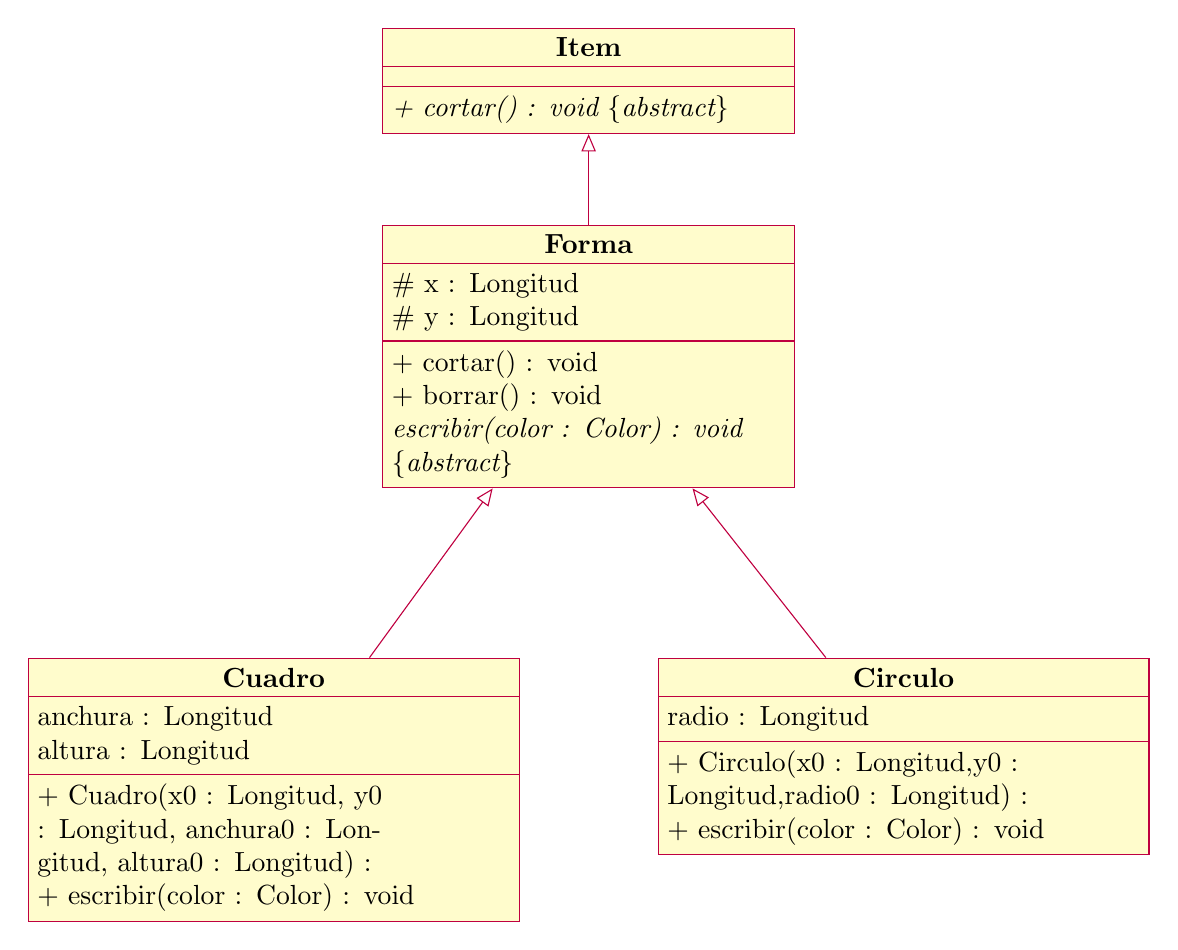
\begin{tikzpicture}
  \begin{class}[text width=5cm]{Item}{0,0}
    \operation[0]{+ cortar() : void $\{$abstract$\}$}
  \end{class}
  \begin{class}[text width=5cm]{Forma}{0,-2.5}
    \inherit{Item}
    \attribute{\# x : Longitud}
    \attribute{\# y : Longitud}
    \operation{+ cortar() : void }
    \operation{+ borrar() : void}
    \operation[0]{escribir(color : Color) : void $\{$abstract$\}$}
  \end{class}
  \begin{class}[text width=6cm]{Cuadro}{-4,-8}
    \inherit{Forma}
    \attribute{anchura : Longitud}
    \attribute{altura : Longitud}
    \operation{+ Cuadro(x0 : Longitud, y0 : Longitud, anchura0 : Longitud, altura0 : Longitud) : }
    \operation{+ escribir(color : Color) : void}
  \end{class}
  \begin{class}[text width=6cm]{Circulo}{4,-8}
  \inherit{Forma}
  \attribute{radio : Longitud}
  \operation{+ Circulo(x0 : Longitud,y0 : Longitud,radio0 : Longitud) : }
  \operation{+ escribir(color : Color) : void}
  \end{class}
\end{tikzpicture}
\end{center}
%En pr\'{o}ximas versiones de este documento se mostrar\'{a}n esqueletos de c\'{o}digo, a partir 
%de los cuales se podr\'{a} construir la versi\'{o}n del programa aqu\'{i} descrito.
\section*{Archivos fuente de la versi\'{o}n inicial}
En los archivos {\tt .h} se han colocado las declaraciones de los tipos de datos uint, Longitud, 
Color, Forma, Cuadro y Circulo. De estos, uint, Longitud y Color son declarados usando {\tt typedef}; 
mientras que Forma, Cuadro y Circulo son clases de objetos. La clase base Forma tiene un m\'{e}todo 
virtual puro (el m\'{e}todo {\tt void escribir(Color)}), por lo tanto, es una clase abstracta; las clases 
Cuadro y Circulo son clases derivadas de la clase Forma. La clase Cuadro se utiliza para representar 
rect\'{a}ngulos y la clase Circulo se utiliza para representar circunferencias. En estas dos clases, 
el m\'{e}todo virtual {\tt void escribir(Color)} no es puro, y por esta raz\'{o}n debe resolverse en 
las dos clases. Como consecuencia ambas clases son concretas.
\subsection*{Archivos de cabecera}
\begin{verbatim}
/** types.h */
#include <SDL.h>
typedef unsigned int uint;
typedef int Longitud;
typedef Uint32 Color;
\end{verbatim}
\begin{center}
Archivo {\tt types.h}
\end{center}

\begin{verbatim}
/** Forma.h */
#include <SDL.h> /* Add -I/usr/include/SDL/ in <command line>/<make file> */
#include <types.h>
#ifndef FORMA_H
#define FORMA_H
class Forma{
protected:
  Longitud x;
  Longitud y;
static SDL_Surface *screen;
public:
  Forma();
  Forma(Longitud x0,Longitud y0);
  void borrar();
static void set_sdl_surface(SDL_Surface *);
static SDL_Surface *get_sdl_surface();
virtual void escribir(Color color)=0;
};/*end class Forma*/
#endif /*FORMA_H*/
\end{verbatim}
\begin{center}
Archivo {\tt Forma.h}
\end{center}

\begin{verbatim}
/** Cuadro.h */
#include <Forma.h>
#ifndef CUADRO_H
#define CUADRO_H
class Cuadro : public Forma{
  Longitud anchura;
  Longitud altura;
public:
  Cuadro();
  Cuadro(Longitud x0,Longitud y0,
         Longitud anchura0,Longitud altura0);
  void escribir(Color color);
};/*end class Cuadro*/
#endif /*CUADRO_H*/
\end{verbatim}
\begin{center}
Archivo {\tt Cuadro.h}
\end{center}

\begin{verbatim}
/** Circulo.h */
#include <Forma.h>
#ifndef CIRCULO_H
#define CIRCULO_H
class Circulo : public Forma{
  Longitud radio;
public:
  Circulo();
  Circulo(Longitud x0,Longitud y0,
          Longitud radio0);
  void escribir(Color color);
};/*end class Circulo*/
#endif /*CIRCULO_H*/
\end{verbatim}
\begin{center}
Archivo {\tt Circulo.h}
\end{center}
\subsection*{Archivos fuente}
A continuaci\'{o}n se incluyen los c\'{o}digos fuente (C++) de los archivos 
{\tt Forma.cpp, Cuadro.cpp, Circulo.cpp, Bresenhamslinealgorithm.cpp, 
Elipse.cpp, escribir.cpp, TestFG.cpp}
\begin{verbatim}
/** Forma.cpp */
#include <Forma.h> /* Add -I./include in <command line>/<make file> */
Forma::Forma(){ }

Forma::Forma(Longitud x0,Longitud y0):x(x0),y(y0){ }

SDL_Surface *Forma::screen=NULL;   /*It will be modifyied in main function*/

void Forma::set_sdl_surface(SDL_Surface *sdl_surf_Pt)
{
  screen=sdl_surf_Pt;
}

SDL_Surface *Forma::get_sdl_surface()
{
  return screen;
}
\end{verbatim}
\begin{center}
Archivo {\tt Forma.cpp}
\end{center}
\begin{verbatim}
/** Cuadro.cpp */
#include <Cuadro.h>   /* Add -I./include in <command line>/<make file> */

Cuadro::Cuadro(){ }

Cuadro::Cuadro(Longitud x0,Longitud y0,
               Longitud anchura0,Longitud altura0)
:Forma(x0,y0),anchura(anchura0),altura(altura0){  }
\end{verbatim}
\begin{center}
Archivo {\tt Cuadro.cpp}
\end{center}
\begin{verbatim}
/** Circulo.cpp */
#include <Circulo.h>   /* Add -I./include in <command line>/<make file> */
Circulo::Circulo(){ }

Circulo::Circulo(Longitud x0,Longitud y0,
                 Longitud radio0)
:Forma(x0,y0),radio(radio0){  }
\end{verbatim}
\begin{center}
Archivo {\tt Circulo.cpp}
\end{center}
\begin{verbatim}
/** Bresenhamslinealgorithm.cpp - An implementation of the 
 *  Bresenham's line algorithm. It uses the 
 *  Simple Directmedia Layer (SDL) library.
 *  (Tested with SDL version 1.2 on friday 2020.03.27).
 */
#include <stdio.h>
#include <stdlib.h>
#include <SDL.h>
#include <iostream>
#include <cmath>   /*fabs()*/
//using std::swap;
//typedef int Longitud;
#include <types.h>   /* Add -I./include in <command line>/<make file> */

void swap(int *i, int *j) {
        int t = *i;
        *i = *j;
        *j = t;
}

void draw_pixel(SDL_Surface *surface, Longitud x,
                Longitud y, Uint32 color) {
        // 32bpp pixel address
        Uint8 *p = (Uint8 *)surface->pixels + y * surface->pitch + x * 4;
        // assign color
        *(Uint32 *)p = color;
}

/** Function to draw a line on a SDL_Surface from point (x1,y1) 
 *  to point (x2,y2). Longitud es un tipo definido por el usuario 
 *  (no una clase) que oculta la verdadera implementaci\'on de la 
 *  longitud (de tal modo que pueda ser entera o real, por ejemplo). 
 *  Se puede declarar mediante un typedef como sigue:
 *  typedef int Longitud;
 *  El par\'ametro color de tipo Uint32 se puede obtener usando 
 *  la funci\'on Uint32 SDL_MapRGB(const SDL_PixelFormat * const format,
                        const Uint8 r, const Uint8 g, const Uint8 b); 
 *  de cuyo uso aqu\'i se muestran un par de ejemplos:
 *  Uint32 black = SDL_MapRGB(screen->format, 0x00, 0x00, 0x00); 
 *  Uint32 white = SDL_MapRGB(screen->format, 0xFF, 0xFF, 0xFF);
 *  donde screen es de tipo SDL_Surface *, y como puede comprobarse 
 *  en 
 *  /usr/include/SDL/SDL_video.h, 
 *  screen->format es de tipo SDL_PixelFormat *.
 */
void Line(SDL_Surface *surface,Longitud x1,Longitud y1, 
          Longitud x2, Longitud y2, const Uint32& color )
{
    // Bresenham's line algorithm
    const bool steep = (fabs(y2 - y1) > fabs(x2 - x1));
    if(steep)
    {
        //std::swap(x1, y1);
        //std::swap(x2, y2);
        swap(&x1,&y1);
        swap(&x2,&y2);
    }

    if(x1 > x2)
    {
        //std::swap(x1, x2);
        //std::swap(y1, y2);
        swap(&x1,&x2);
        swap(&y1,&y2);
    }

    const Longitud dx = x2 - x1;
    const Longitud dy = fabs(y2 - y1);

    float error = dx / 2.0f;
    const int ystep = (y1 < y2) ? 1 : -1;
    int y = (int)y1;

    const int maxX = (int)x2;

    for(int x=(int)x1; x<maxX; x++)
    {
        if(steep)
        {
            //SetPixel(y,x, color);
            draw_pixel(surface,y,x,color);
        }
        else
        {
            //SetPixel(x,y, color);
            draw_pixel(surface,x,y,color);
        }

        error -= dy;
        if(error < 0)
        {
            y += ystep;
            error += dx;
        }
    }
}/*end Line()*/
\end{verbatim}
\begin{center}
Archivo {\tt Bresenhamslinealgorithm.cpp}
\end{center}
\begin{verbatim}
/** Elipse.cpp
The code of the function is based on:
Download url:
https://stackoverflow.com/questions/38334081/
howto-draw-circles-arcs-and-vector-graphics-in-sdl
If you want to do a circle or ellipse without 3rd 
party libraries, include math.h and use the function 
below I wrote. It will draw aliased ellipse or circles 
very well. It draws one quadrant arc, and mirrors the 
other arcs, reducing calls to cosf and sinf. */
#include <stdio.h>
#include <stdlib.h>
#include <SDL.h>
#include <iostream>
#include <cmath>   /*fabs()*/
typedef int Longitud;
void Line(SDL_Surface *surface,Longitud x1,Longitud y1, 
          Longitud x2, Longitud y2, const Uint32& color);


//draw one quadrant arc, and mirror the other 4 quadrants
void sdl_ellipse(SDL_Surface* r,int x0,int y0,
                 int radiusX, int radiusY,Uint32 color)
{
    float pi  = 3.14159265358979323846264338327950288419716939937510;
    float pih = pi / 2.0; //half of pi

    //drew  28 lines with   4x4  circle with precision of 150 0ms
    //drew 132 lines with  25x14 circle with precision of 150 0ms
    //drew 152 lines with 100x50 circle with precision of 150 3ms
    const int prec = 27; // precision value; 
                         // value of 1 will draw a diamond, 27 makes 
                         // pretty smooth circles.
    float theta = 0;     // angle that will be increased each loop

    //starting point
    int x  = (float)radiusX * cos(theta);//start point
    int y  = (float)radiusY * sin(theta);//start point
    int x1 = x;
    int y1 = y;

    //repeat until theta >= 90;
    float step = pih/(float)prec; // amount to add to theta 
                                  // each time (degrees)
    //step through only a 90 arc (1 quadrant)
    for(theta=step;  theta <= pih;  theta+=step)
    {
        //get new point location
        //new point (+.5 is a quick rounding method)
        x1 = (float)radiusX * cosf(theta) + 0.5; 
        //new point (+.5 is a quick rounding method)
        y1 = (float)radiusY * sinf(theta) + 0.5; 

        //draw line from previous point to new point, ONLY if point incremented
        if( (x != x1) || (y != y1) )//only draw if coordinate changed
        {
//SDL_RenderDrawLine(r, x0 + x, y0 - y,    x0 + x1, y0 - y1 );//quadrant TR
//SDL_RenderDrawLine(r, x0 - x, y0 - y,    x0 - x1, y0 - y1 );//quadrant TL
//SDL_RenderDrawLine(r, x0 - x, y0 + y,    x0 - x1, y0 + y1 );//quadrant BL
//SDL_RenderDrawLine(r, x0 + x, y0 + y,    x0 + x1, y0 + y1 );//quadrant BR
            Line(r, x0 + x, y0 - y,    x0 + x1, y0 - y1,color);//quadrant TR
            Line(r, x0 - x, y0 - y,    x0 - x1, y0 - y1,color);//quadrant TL
            Line(r, x0 - x, y0 + y,    x0 - x1, y0 + y1,color);//quadrant BL
            Line(r, x0 + x, y0 + y,    x0 + x1, y0 + y1,color);//quadrant BR
        }
        //save previous points
        x = x1;//save new previous point
        y = y1;//save new previous point
    }
    //arc did not finish because of rounding, so finish the arc
    if(x!=0)
    {
        x=0;
//SDL_RenderDrawLine(r, x0 + x, y0 - y,    x0 + x1, y0 - y1 );//quadrant TR
//SDL_RenderDrawLine(r, x0 - x, y0 - y,    x0 - x1, y0 - y1 );//quadrant TL
//SDL_RenderDrawLine(r, x0 - x, y0 + y,    x0 - x1, y0 + y1 );//quadrant BL
//SDL_RenderDrawLine(r, x0 + x, y0 + y,    x0 + x1, y0 + y1 );//quadrant BR
        Line(r, x0 + x, y0 - y,    x0 + x1, y0 - y1,color);//quadrant TR
        Line(r, x0 - x, y0 - y,    x0 - x1, y0 - y1,color);//quadrant TL
        Line(r, x0 - x, y0 + y,    x0 - x1, y0 + y1,color);//quadrant BL
        Line(r, x0 + x, y0 + y,    x0 + x1, y0 + y1,color);//quadrant BR
    }
}/*end sdl_ellipse()*/
\end{verbatim}
\begin{center}
Archivo {\tt Elipse.cpp}
\end{center}
\begin{verbatim}
/** escribir.cpp */
#include <Cuadro.h>
#include <Circulo.h>
void Line(SDL_Surface *surface,Longitud x1,Longitud y1, 
          Longitud x2, Longitud y2, const Color& color );
void sdl_ellipse(SDL_Surface* r,Longitud x0,Longitud y0, 
                 Longitud radiusX,Longitud radiusY,Color color);

void Cuadro::escribir(Color color)
{
  Longitud pX,pY,b,a;
  pX=3*x/4;pY=y;
  a=altura;
  b=3*anchura/4;
  Line(Forma::screen,pX,pY,pX+b,pY,color);
  Line(Forma::screen,pX+b,pY,pX+b,pY+a,color);
  Line(Forma::screen,pX+b,pY+a,pX,pY+a,color);
  Line(Forma::screen,pX,pY+a,pX,pY,color);
}

void Circulo::escribir(Color color)
{
  Longitud pX,pY,radX,radY;
  pX=3*x/4;pY=y;
  radX=3*radio/4;
  radY=radio;
  sdl_ellipse(Forma::screen,pX,pY,radX,radY,color);
}
\end{verbatim}
\begin{center}
Archivo {\tt escribir.cpp}
\end{center}
\begin{verbatim}
/** TestFG.cpp */
#include <iostream>
#include <stdio.h>
using namespace std;
#include <Cuadro.h>
#include <Circulo.h>
/*
SOLVING ERROR: undefined reference to 'vtable...
The solution is to ensure that all virtual methods 
that are not pure are defined. Note that a destructor 
must be defined even if it is declared pure-virtual 
[class.dtor]/7
*/

int main(int argc,char *argv[])
{
  SDL_Event event;
  int done = 0;
  printf("Initial test...\n");
  // Inicializamos SDL
  if (SDL_Init(SDL_INIT_VIDEO) < 0) {
    printf("No se pudo iniciar SDL: %s\n",SDL_GetError());
    return 1;
  }
  // Inicializamos los objetos
  Cuadro *Q1=new Cuadro(200,200,200,200);
  Circulo *C1=new Circulo(200,200,100);

  // Inicializamos modo de video
  Forma::set_sdl_surface(
         SDL_SetVideoMode(640,480,24,
         SDL_HWSURFACE|SDL_DOUBLEBUF|SDL_RESIZABLE));
  if (NULL==Forma::get_sdl_surface()) {
   printf("No se puede inicializar el modo gr\\'afico: \n",SDL_GetError());
   return 1;
  }
  atexit(SDL_Quit);
  
 // Dibujamos las figuras
  Color white = SDL_MapRGB(Q1->get_sdl_surface()->format, 0xFF, 0xFF, 0xFF);
  Q1->escribir(white);
  C1->escribir(white);
  SDL_Flip(Forma::get_sdl_surface());            /*Added by LMC 2020.03.26*/

  // Esperamos la pulsaci\'on de una tecla para salir
  while(done == 0) {
    while ( SDL_PollEvent(&event) ) {
      if ( event.type == SDL_KEYDOWN ) 
       done = 1;
    }
  }

  return 0;
}/*end main()*/
\end{verbatim}
\begin{center}
Archivo {\tt TestFG.cpp}
\end{center}
El archivo make utilizado para construir el archivo ejecutable 
es el siguiente
\begin{verbatim}
EXE0:=00_TestFigurasGeometricas_SDL.exe
TEST:=$(EXE0)
LIMPIEZA:= *.o $(TEST)
OBJETOS:=Cuadro.o\
         Circulo.o\
         Forma.o\
         TestFG.o\
         Bresenhamslinealgorithm.o\
         Elipse.o\
         escribir.o\

CC=g++
#CXXFLAGS += -I./include/ -I/usr/include/SDL/ -D_GNU_SOURCE=1 -D_REENTRANT
CXXFLAGS += -I./include/ -I/usr/include/SDL/ 
LDFLAGS += -lSDL 
default:$(TEST)
$(EXE0):$(OBJETOS)
	$(CC) $(LDFLAGS) $^ -o $@
clean:
	rm -v $(LIMPIEZA)
\end{verbatim}
\begin{center}
Archivo Makefile
\end{center} 
\end{document}